\documentclass[]{article}
\usepackage{graphicx}
\usepackage[labelformat=empty]{caption}

\begin{document}

% bacterial expression

% eukaryote expression

% forward genetics 20

% reverse genetics 10

% TEs 10

% genomics

%popgen 20
%quantgen

%organellar genomes 10


The first five problems below refer to the \emph{zombiedefense} locus in the brainplant species.  At this locus, brainplants with the dominant allele D are immune to zombie disease. Vulnerable homozygous recessive dd brainplants die from a mysterious zombie sickness when bitten by zombies.  

\begin{enumerate}

\item You sample 125 brainplants from a population. You take them back to the lab and have a zombie bite them.  5 are vulnerable and 120 are immune. If this population is at Hardy-Weinberg Equilibrium, what is the frequency of the D allele? (10 pts)

\bigspace}

%0.8, the d allele is 0.2

\item If zombie attacks are frequent in nature, the D allele should eventually reach 100\% frequency (i.e. fix) in the population.  Why will it take a long time to fix? (10 pts)

% because removing recessive deleterious alleles is hard since most hang out in hets

\item In your greenhouse populations you observe a new recessive mutant which you call the \emph{ouch} mutant.  Plants homozygous for the \emph{o} allele at this locus are also killed by zombie bites.  You cross individuals homozygous for each of the mutants.  Write out the genotypes of the two individuals if:
\begin{enumerate}
\item all the progeny result immune (5pts)
% oo DD x OO dd (two loci)
\item all the progeny result vulnerable (5pts).
% dd x dd  (one locus)
\end{enumerate}

\item The \emph{yummy} locus codes for a protein that attracts zombies. Below is a pedigree of plants and their phenotypes for at the \emph{zombiedefense} and \emph{yummy} loci. Filled shapes represent plants with the yummy phenotype, and plants with stars represent those vulnerable to zombie bites. In brainplants the mitochondria is paternally inherited.  

\begin{enumerate}
\item What can you say about the genetic basis of the \emph{yummy} locus? (5pts)

%chloroplast

\item Brainplants are hemaphroditic. If the first cross had been done in reverse and the vulnerable parent was used as the maternal plant, draw an arrow to all plants on the pedigree that would show the yummy phenotype. (5pts)

%none

\end{enumerate}

\begin{figure}[here]
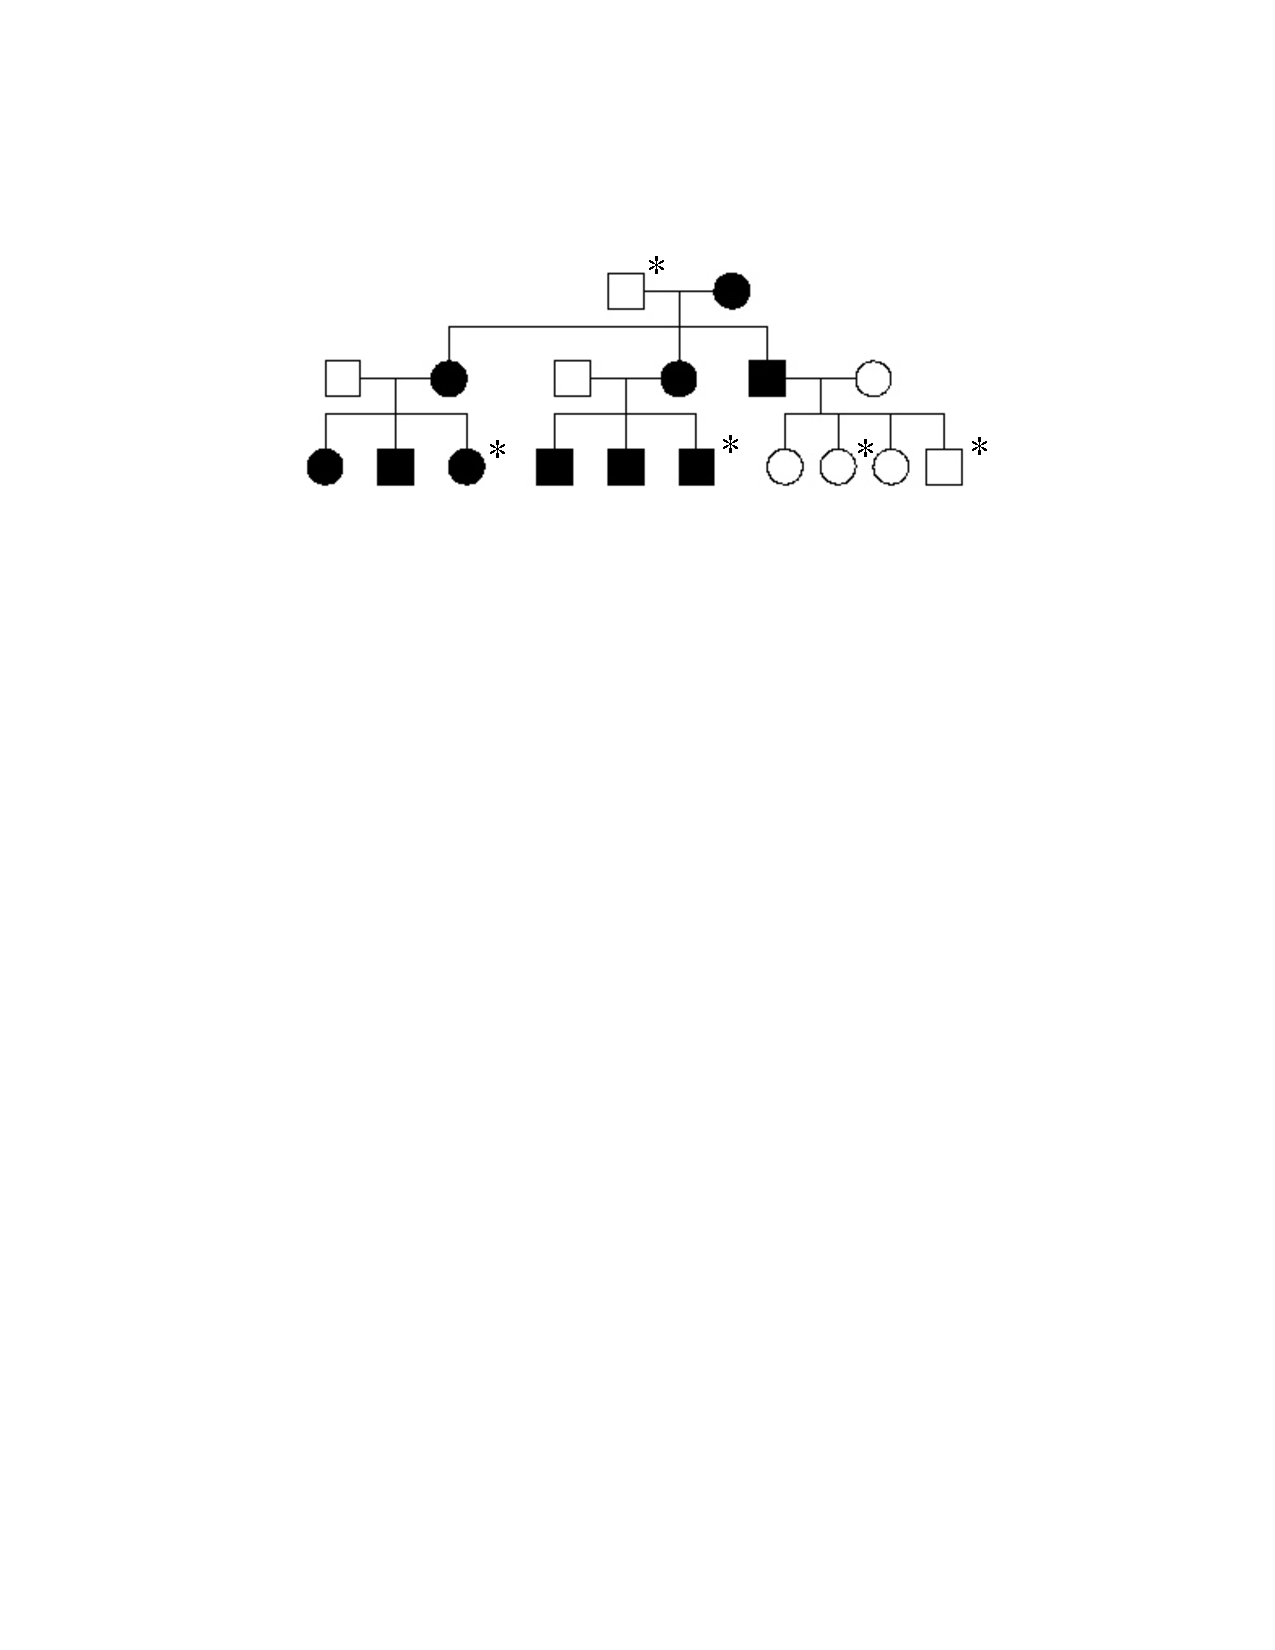
\includegraphics[width=12cm]{pedigree.pdf}
\caption{}
\label{fig:ped}
\end{figure}

\item You want to map the \emph{zombiedefense} locus. You make use of a nonautonomous DNA element called zap and the related autonomous element pow. You take a single plant immune to zombie bites and cross it with itself. The plant's genotype (zap+ means presence of zap, and pow- means absence of pow) is:  D zap+ / d zap- ; pow+ / pow+  .  Will there be more or fewer vulnerable plants among the progeny?  Why? (10pts)

%more, zap jumps into D.



 

\end{enumerate}

The next five problems refer to puffybunnies, the world's cutest animal. Unfortunately, puffybunnies are commonly infected with a disease that makes them lose all their hair. 

\begin{enumerate}

\item 

\end{enumerate}






\end{document}